\documentclass[11pt]{article}
\usepackage{graphicx}
\usepackage{enumitem}

\begin{document}

\section{Implementation}
In this section we present our implementation of LDA in python and discuss our results.
\subsection{Library Used}
	
    \begin{itemize}[noitemsep]
		\item numpy
		\item scikit learn for pre-processing
		\item scipy probability distributions
 	\end{itemize}
\subsection{Dataset Description}
The dataset used is the same one used in the authors implementation. it can be found at the following link: \texttt{ https://nlp.stanford.edu/software/tmt/tmt-0.4/}
It consist of 2246 small documents. 
   
\subsection{Pre-processing}
\textbf{Tokenization of the documents:}  LDA use the bag of word assumption (the order of words apparitions in a document is ignored). This allows us to use a compact representation of every documents in a matrix of M x V.  Each line in the matrix represent a document and the values are integer that represent the number of occurrence of a word in the vocabulary. This is similar to the one hot encoding trick that we used in the class. \\
\\
In addition  to tokenization, we included the following filters to remove words that have either a too low or too high frequency: 
    \begin{itemize}[noitemsep]
		\item Removed  words with only 1 occurrence across the corpus.
		\item Removed words that occur in 95 \% of the document or more. 
	\end{itemize}
\subsection{Parameter Initialization}
As stated in section xxxx, LDA with with variational EM has 4 set of parameters to estimate, each  of the parameters are randomly initialized to the following value:

\begin{tabular}{ |p{2cm}||p{3cm}|p{10cm}| }
 \hline
 Parameter & Dimension  & Initialization\\
 \hline
  $\alpha$ & [K]   & np.random.gamma(shape=np.ones((K)), scale=1/K)\\
  $\phi$  & [M x N[d] x K]  & 1 / K * np.ones((N[d], K)) (per doc)\\
  $\beta$  & [K x V]  &  np.random.dirichlet(np.ones(V), K)\\
  $\gamma $  & [M x K]  &  alpha + np.max((N[d] / K, 0.2)) \\
  \hline
\end{tabular}\\
\\
We added a second term to the innitial $\gamma $ to ensure that we dont encounter overflow in the first iterations of the variational inference algorithm.
\\
\subsection{Stopping Criterion}
In the paper, the author doesn't state very clearly the stopping criterion used in its implementation. So we chose to stop the model once the parameter L2 norm of $\gamma$   from one iteration to the next is is below a given threshold. 
\\
stopping metric:
in the paper

\begin{figure}[ht]
\vskip 0.2in
\begin{center}
\centerline{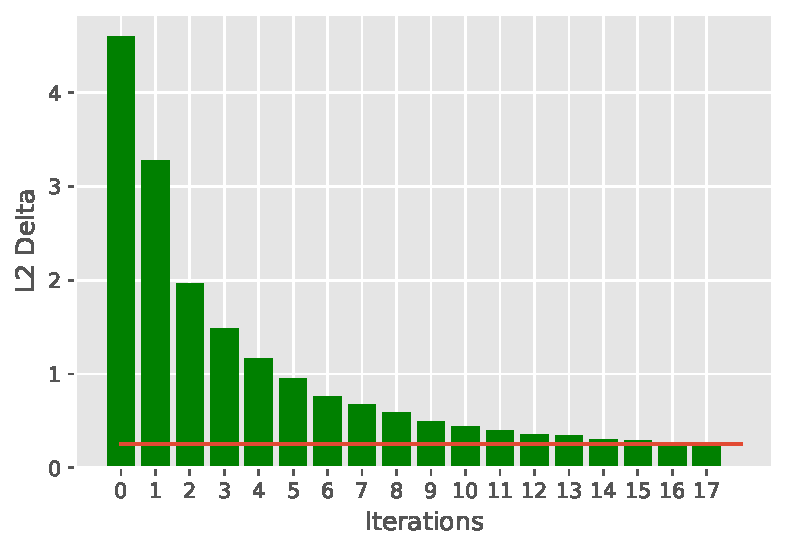
\includegraphics[width=\columnwidth]{plot_delta_gamma_convergence}}
\caption{Change in $\gamma$ parameter across EM iterations. The green bars represent the L2 change of  $\gamma$ parameters. The red line represent the stopping criterion  used (0.25 in our case).}
\label{icml-historical}
\end{center}
\vskip -0.2in
\end{figure}

\subsection{Results}
%here is a sample of 5 topics from our implemtention with the top 10 words from 
\begin{table}[h]
\caption{Topic Sample from LDA model: each column represent the top 10 words from the topic }

  \scalebox{0.6}{
    \begin{tabular}
    { |p{2cm}|p{2cm}|p{2cm}|p{2cm}|p{2cm}| }
 \hline
 \multicolumn{5}{|c|}{Topic Sample} \\
 \hline
 Topic 1 & Topic 2  &  Topic 3 & Topic 4 & Topic 5\\
 \hline
 club & new & child & ago & american\\
 year & percent & people & africa & states\\
 york & yen & having & leaders & union\\
 old & economy & report & france & told\\
 building & rate & education & people & political\\
 business & rates & aids & african & leaders\\
 years & said & children & french & conference\\
 new & prices & said & south & president\\
 city & market & care & police & said\\
 said & dollar & health & said & soviet\\
 \hline
\end{tabular}}
\end{table}
\end{document}
